\section{Fattori e indicatori di una Smart City}
Il Centro per la globalizzazione e la strategia della IESE Business School dell'università di Navarra, in particolare IESE Cities in Motion\footnote{Cities in Motion è una piattaforma di ricerca lanciata congiuntamente dal CGS Center for Globalizaton and Strategy e da IESE Business School entrambi dell'università di Navarra, la cui missione è di creare un approccio innovativo alle città e un nuovo modello urbano per il XXI secolo basato su quattro fattori principali: ecosistema sostenibile, attività creative, uguaglianza tra cittadini e connessione del territorio}, nel 2019 ha stilato una classifica delle dieci migliori città Smart City del mondo basandosi su nove aspetti fondamentali.\cite{iese_cities_2019}
L'obiettivo di questo lavoro è di promuovere i cambiamenti a livello locale e sviluppare idee preziose e strumenti innovativi che porteranno le città ad essere più sostenibili e più intelligenti. 

\todo{gdm: motivare i vari fattoroi e indicatori - perchè questi fanno una sm rispetto ad una city}

\subsection{Economia}
Sono incluse tutte le politiche economiche di una amministrazione pubblica. Tenendo conto del grado di diffusione delle nuovitecnologie e servizi che ne emergono, vengono prese in considerazioni anche i servizi digitali non promossi dalle amministrazioni locali quali Glovo, Uber o MyTaxi.
In figura 1.3 sono rappresentati gli indicatori economici.
\begin{figure}[h!]
	\begin{center}
		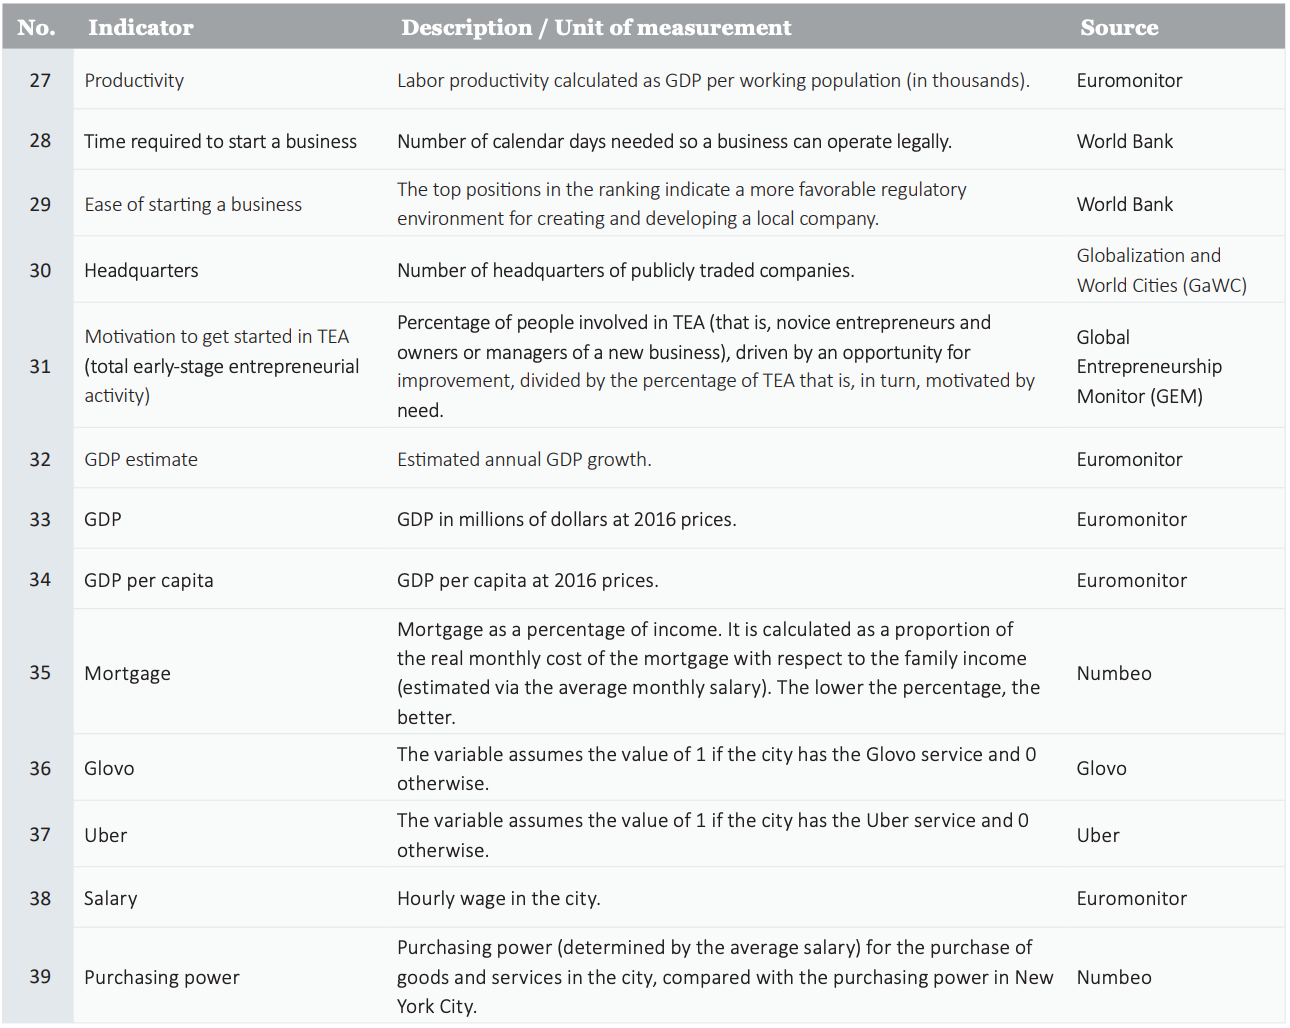
\includegraphics[width=320bp]{img/indicatori_economici.png}
		\caption{Indicatori economici}
	\end{center}
\end{figure}

\subsection{Capitale umano}
Le Cità che intendono avviarsi verso una conversione a Smart City devono essere in grado di attrarre e trattenere talenti, creare piani per migliorare l'istruzione e promuovere sia la creatività che la ricerca e migliora il livello di istruzione dei propri cittadini e l'accesso alla cultura (tenendo conto del numero di musei aperti, gallerie d'arte, librerie e spazi dedicato al tempo libero).
In figura 1.1 sono rappresentati gli indicatori relativi al capitale umano.
\begin{figure}[ht]
	\begin{center}
		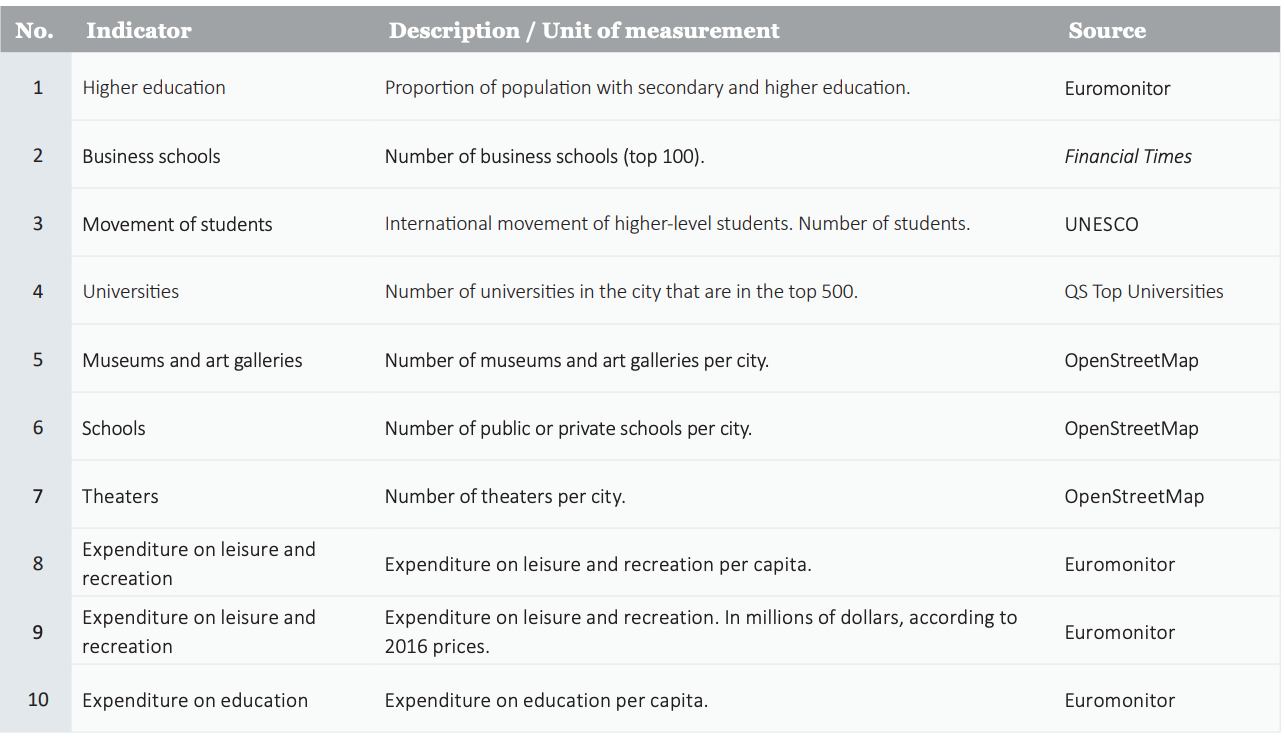
\includegraphics[width=320bp]{img/indicatori_capitale_umano.png}
		\caption{Indicatori capitale umano}
	\end{center}
\end{figure}

\subsection{Politiche sociali}
Per politiche sociali si intende la capacità di coesistenza tra gruppi di persone con redditi, culture, età e professioni diverse che vivono in una città. Inteso anche come il grado di consenso tra i membri di un gruppo sociale o la percezione dell'appartenenza ad una situazione o progetto comune. Viene considerata come un indice per misurare l'interazione sociale all'interno di un gruppo. Inoltre sono visti come segno positivo il numero di centri sanitari pubblici e privati, intesi come servizi sociali di buon aiuto. Come eventi sfavorevoli giudicati come segno negativo sono inclusi gli ati terroristici subiti negli ultimi tre anni.
In figura 1.2 sono rappresentati gli indicatori relativi alle politiche sociali.
\begin{figure}[ht]
	\begin{center}
		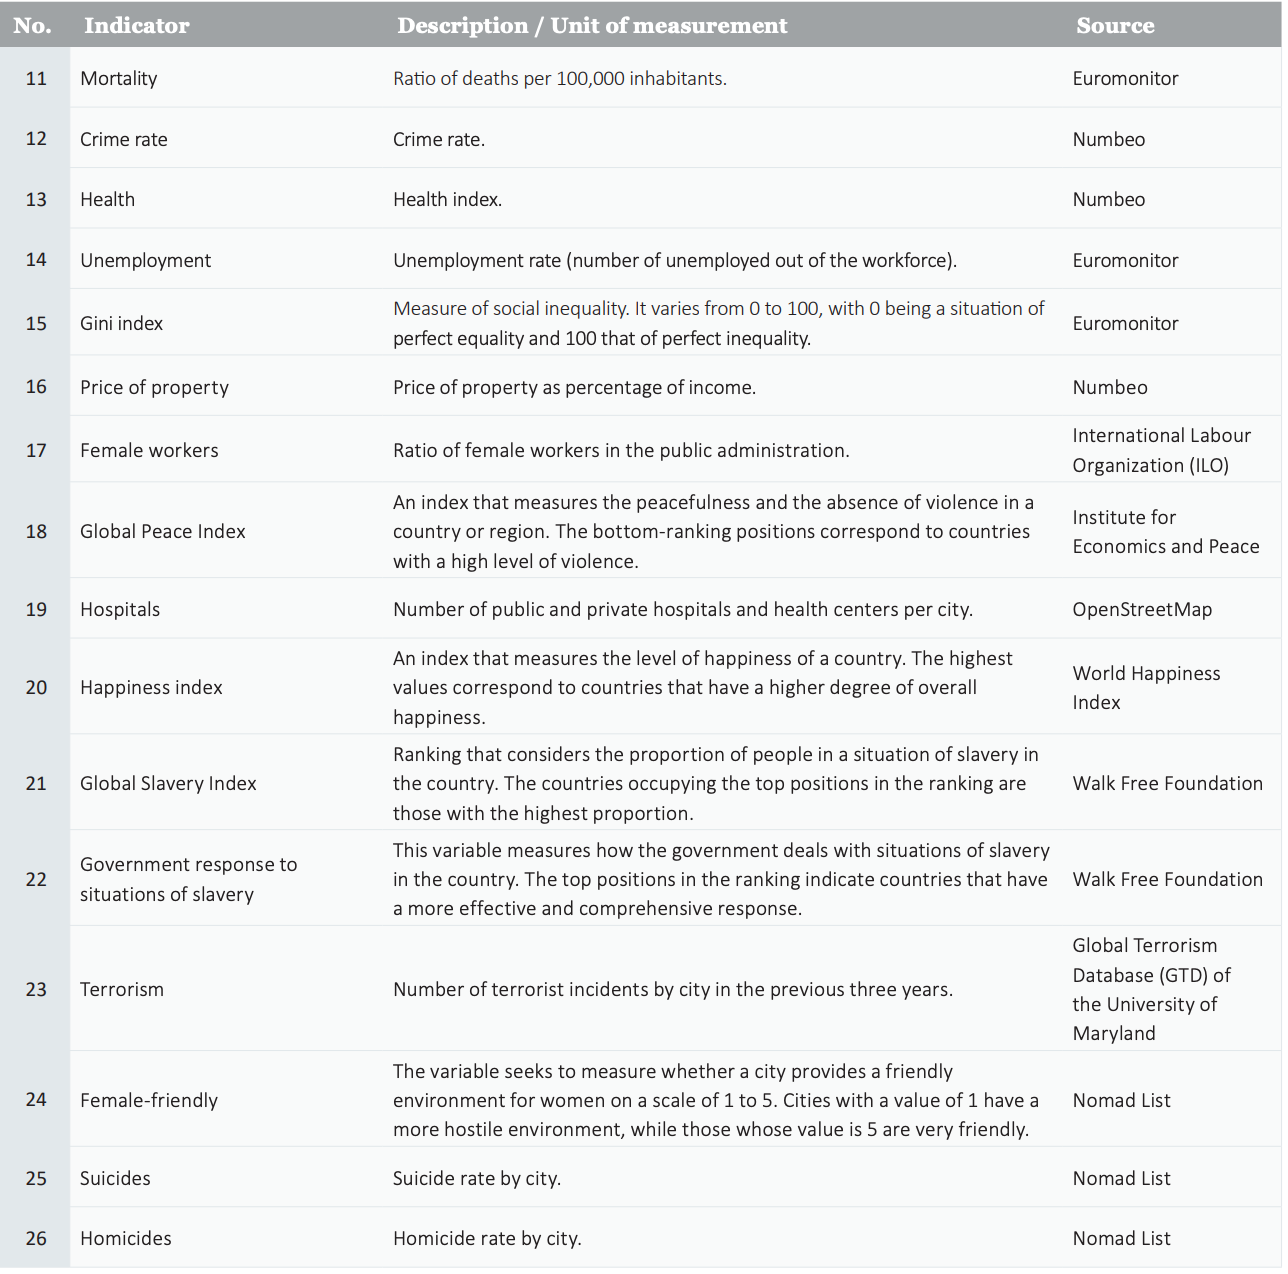
\includegraphics[width=320bp]{img/indicatori_coesione_sociale.png}
		\caption{Indicatori politiche sociali}
	\end{center}
\end{figure}

\subsection{Governance}
Nel lavoro svolto dalla EISE Business School, la governance è considerata come la capacità da parte delle amministrazioni pubbliche locali di amministrare  e di investire i soldi dei contribuenti in politiche volte al miglioramento della qualità della vita del cittadino.
In figura 1.5 vi è la lista degli indicatori per misurare la governance di una Smart City, uni di questi indicatori è la certificazione ISO37120\footnote{La certificazione ISO37120 sancisce un insieme di regole per guidare e misurare le prestazioni dei servizi cittadini e la qualità della vita, questa certificazione può essere applicata a qualsiasi città, comune o governo locale che si impegna a misurare le proprie prestazioni in modo comparabile e verificabile, indipendentemente dalle dimensioni e dalla posizione.} è un forte indicatore in materia di governance per le Smart City, unb altro indicatore è dato dalla percentuale si cittadini occupata nella pubblica amministrazione e nella difesa; formazione scolastica; salute; attività di comunità, servizi sociali e personali; e altre attività.
\begin{figure}[ht]
	\begin{center}
		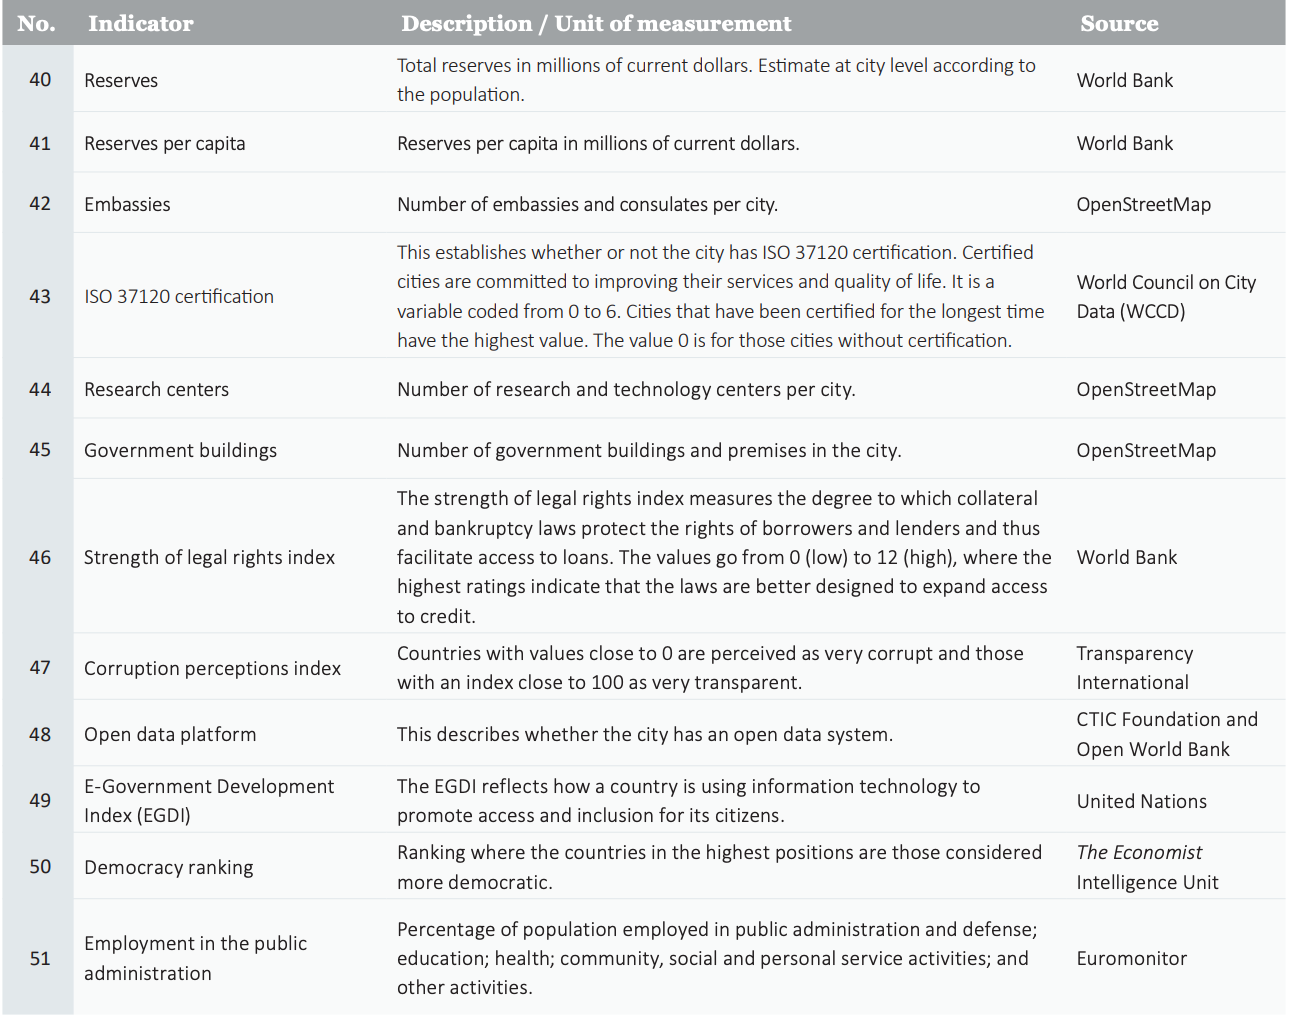
\includegraphics[width=320bp]{img/indicatori_governance.png}
		\caption{Indicatori di governance}
	\end{center}
\end{figure}

\subsection{Ambiebte}
Sono inclusi tutti quei fattori che migliorano la sostenibilità della città come la creazione di edifici ecologici o di classe energetica A superiore, gestione efficiente dell'acqua e dei rifiuti. Tra gli indicatori sono inclusi la qualità dell'aria e dell'acqua che sono anche indicatori della qualità della vita del cittadino. Ridurre i valori di questi indicatori è sopratutto uno degli obiettivi del protocollo di Kyoto.\footnote{Il protocollo di Kyoto è un trattato internazionale in materia ambientale riguardante il surriscaldamento globale, redatto l'11 dicembre 1997 nella città giapponese di Kyoto da più di 180 Paesi}
In figura 1.4 sono rappresentati gli indicatori ambientali.
\begin{figure}[ht]
	\begin{center}
		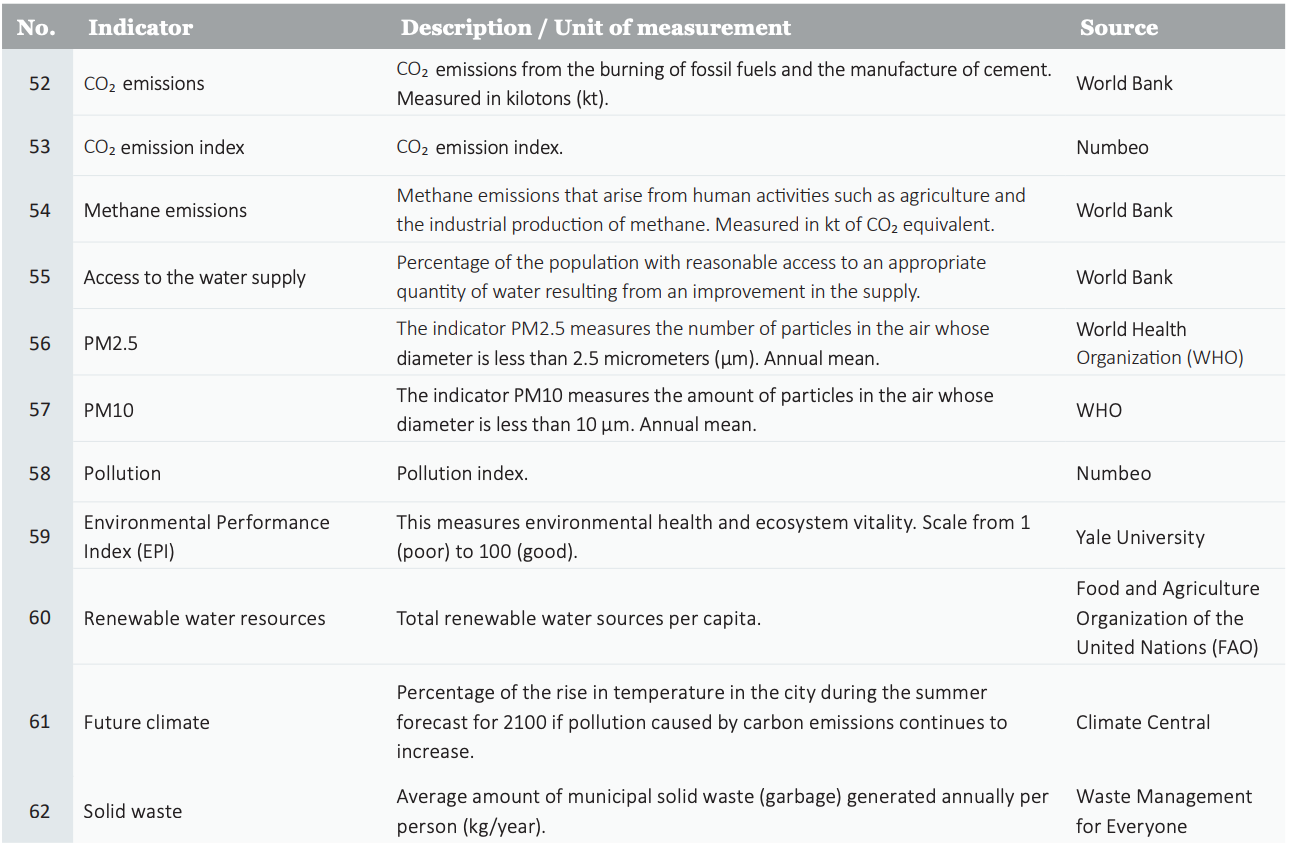
\includegraphics[width=320bp]{img/indicatori_ambientale.png}
		\caption{Indicatori ambientali}
	\end{center}
\end{figure}


\subsection{Pianificazione urbana}
Per pianificazione urbana si intende l'insieme dei servizi pubblici volti a migliorare l'abitabilità della città e quindi ad aumentare la qualità della vita del cittadino. Tra gli indicatori, per una buona pianificazione di abitabilità, vi è la presenza di bike sharing, ovvero il numero di punti di stazione di bikesharing presenti nel territorio, altri indicatori sono rappresentati in figura 1.6.
\begin{figure}[ht]
	\begin{center}
		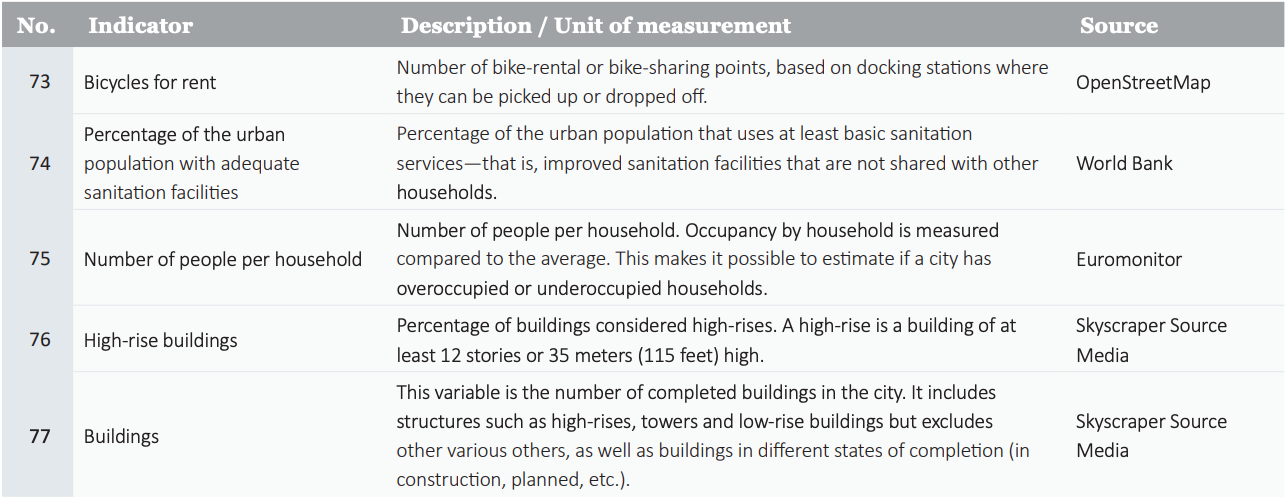
\includegraphics[width=320bp]{img/indicatori_pianificazione_urbana.png}
		\caption{Indicatori di pianificazione urbana}
	\end{center}
\end{figure}

\subsection{Sensibilizzazione internazionale}
Per sensibilizzazione internazionale si intende la capacità di una città di offrire tutti quei servizi strategicy volti a far transitare o a permanere il turista nel territorio. Tra gli indicatori vi è il numero di aereoporti e numero di passeggeri per aereoporto, il numero di congressi che si tengono in città e il . numero di alberghi. Il IESE Cities Motion utilizza i dati di \textit{Sightsmap.com}\footnote{Sightsmap.com è un servizio web che mostra la popolarità di un luogo basandosi sul numero di foto panoramiche scattate.} come indicatore per ottenere il grado di popolarità di un luogo. In figura 1.7 la lista degli altri indicatori.
\begin{figure}[ht]
	\begin{center}
		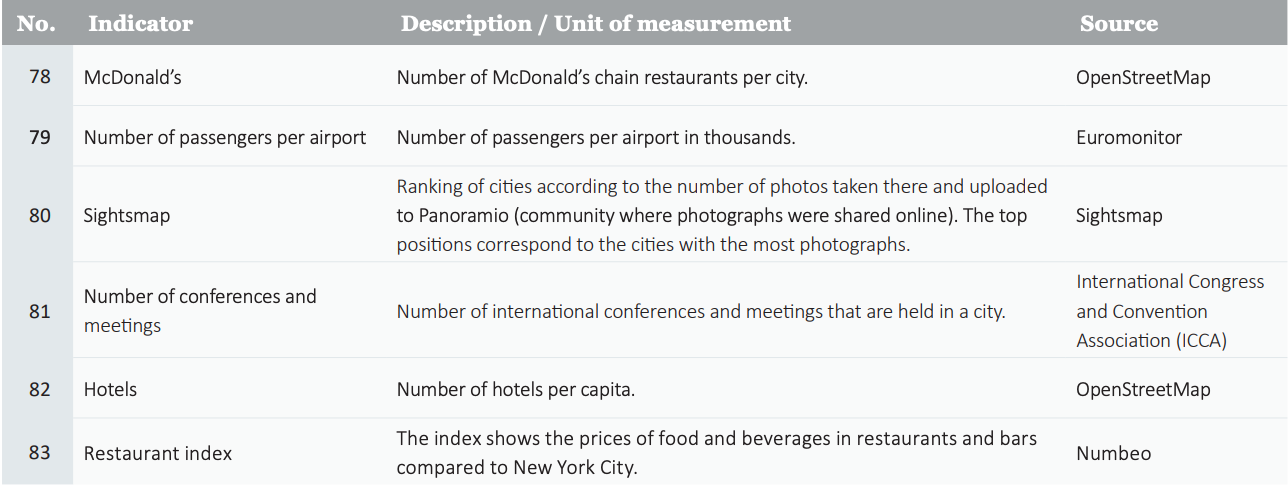
\includegraphics[width=320bp]{img/indicatori_sensibilizzaqzione_internazinale.png}
		\caption{Indicatori di sensibilizzazione internazionale}
	\end{center}
\end{figure}


\subsection{Tecnologia}
L'aspetto tecnologico, per una città che intende evolversi in Smart City, è il fattore fondamentale da tenere in considerazione. Tra gli indicatori tecnologici che sono visti positivamente in una Smart City sono il numero di Hotspot WiFi\footnote{Un Hotspot è un luogo coperto da una connessione pubblica aperta a tutti.} sparsi per la città, la percentuale di famiglie connesse a internet e la percentuale di famiglie che possiede un pc. L'introduzine nella società di queste tecnologie può causare uno sgradevole fenomeno all'inerno di una Città ovvero può  creare il cosidetto \textit{digital divide}\footnote{Dall'enciclopedia Treccani: il digital devide è un espressione nata in seno all’amministrazione statunitense della presidenza Clinton (1993-2001) per indicare la disparità nelle possibilità di accesso ai servizi telematici tra la popolazione americana e sta ad indicare la consapevolezza globale di una problematica di accesso ai mezzi di informazione e comunicazione da parte di determinate aree geografiche o fasce di popolazion},\cite{problem_smar_city_digitaldivide} è compito delle politiche sociali di una amministrazione pubblica fare in modo che questo fenomeno non si evolvi. \cite{iese_cities_2019}
l'IESE Citie Motion, tra gli indicatori, tiene conto anche dell'attività dei cittadini sui social in particolare Twetter\footnote{Twitter è un servizio di notizie e microblogging fornito dalla società Twitter, Inc. su cui gli utenti postano[2] e interagiscono con messaggi chiamati tweet. La Twitter, Inc. ha sede in San Francisco (Stati Uniti)} e Linkedin\footnote{LinkedIn è un servizio web di rete sociale, gratuito, rivolto principalmente nello sviluppo di contatti professionali e nella diffusione di contenuti specifici relativi al mercato del lavoro (es. motore di ricerca del lavoro, pubblicità aziende, ecc.)}.
In figura 1.8 è rapresentata la tabella completa di tutti gli altri indicatori tecnologicy.
\begin{figure}[ht]
	\begin{center}
		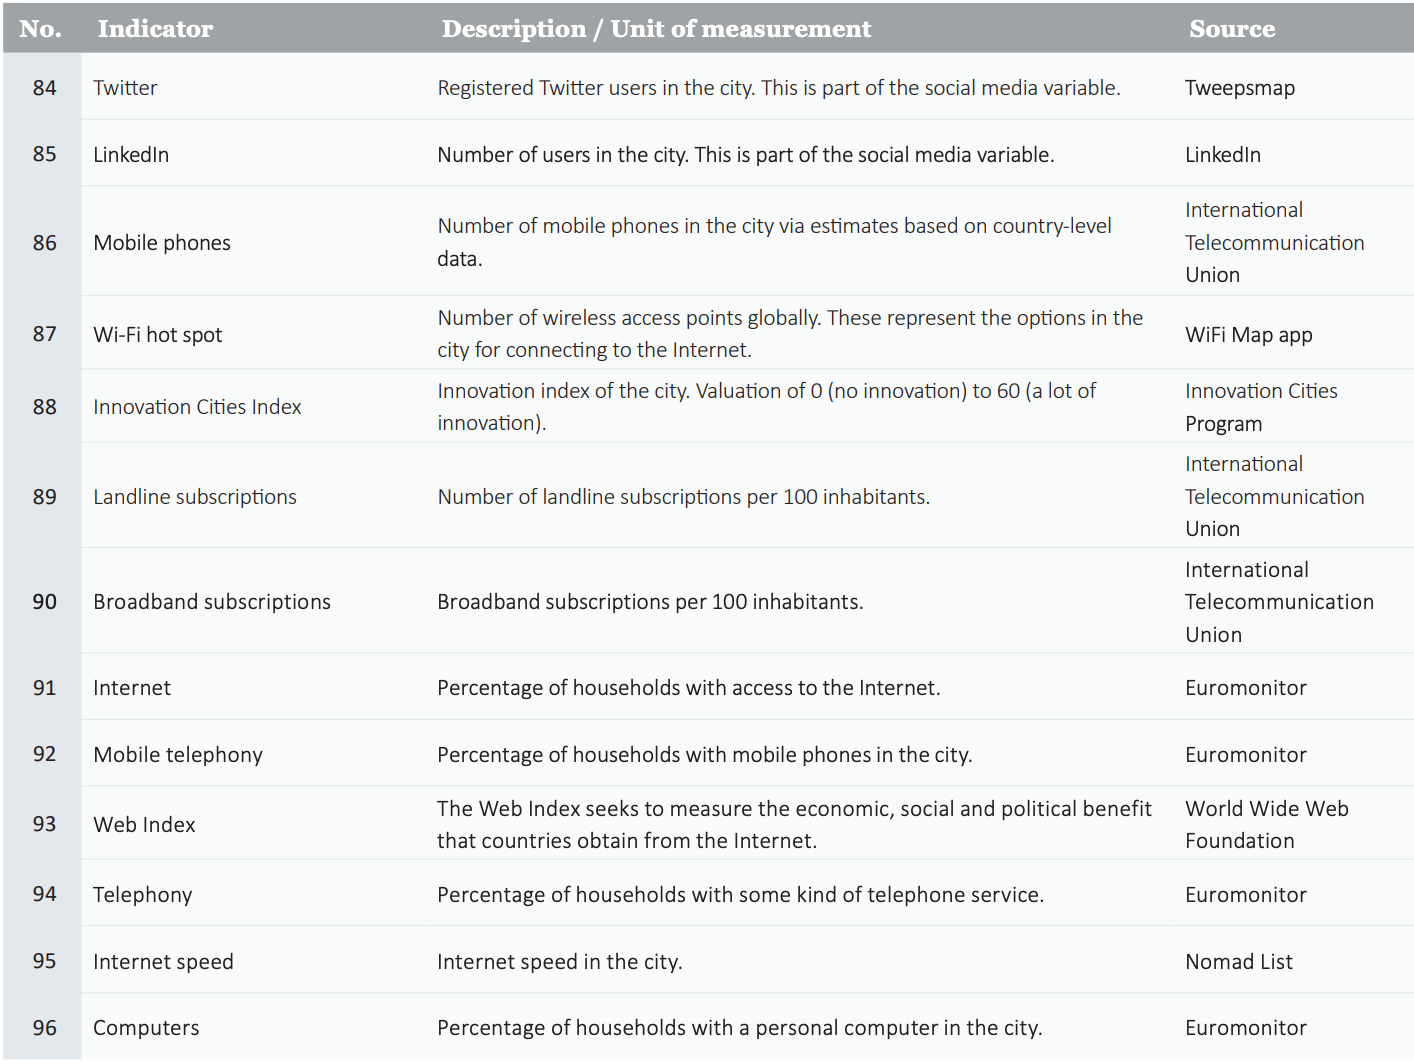
\includegraphics[width=320bp]{img/indicatori_tecnologici.png}
		\caption{Indicatori tecnologici}
	\end{center}
\end{figure}

\subsection{Mobilità e trasporto urbano}
Agevolare il movimento all'interno della città, il numero di mezzi pubblici e il loro accesso è un altro fattore importante che non può mancare in una Smart City. Gli indicatori di questa categoria sono il numero stazioni della metropolitana, l'indice del traffico, qui ritroviamo dinuovo il numero di Bikesharing ecc.
In figura 1.9 tutti gli altri indicatori.
\begin{figure}[ht]
	\begin{center}
		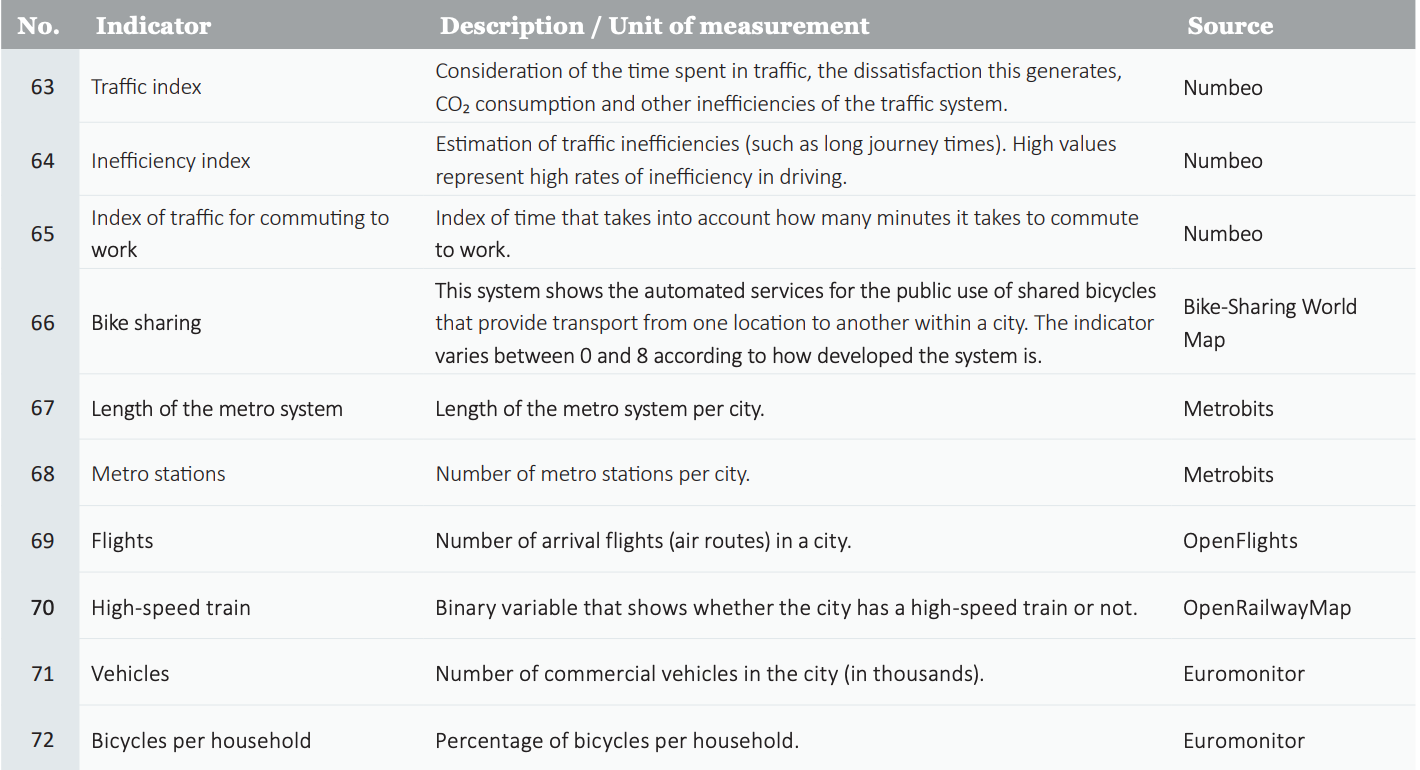
\includegraphics[width=320bp]{img/indicatori_trasporti_urbani.png}
		\caption{Indicatori di mobilità e trasporto urbano}
	\end{center}
\end{figure}